\newpage
\section{Harmonogram pracy}

\subsection{Podział projektu na etapy i zadania}

Prace projektowe odbywają się w trzech iteracjach.

\subsubsection{Iteracja A -- Przygotowanie}
Ogólnym celem iteracji A jest przygotowanie zespołu do prac nad produktami
projektu. Iteracja zakłada:
\begin{itemize}[nosep]
     \item ustalenie wspólnej wizji projektu,
     \item uzyskanie specjalistycznej wiedzy przez zespół,
     \item stworzenie podstawowej dokumentacji,
     \item utworzenie środowiska pracy.
 \end{itemize}

\noindent Planowane rozpoczęcie iteracji A jest na 1. października 2012, z
końcem prac 3. listopada 2012. Budżet iteracji wynosi 40 000 PLN. Harmonogram
wykonania zadań wchodzących w skład iteracji \emph{Przygotowanie} zaczyna się na
stronie \pageref{fig:harmonogram:iteracja_przygotowanie}.

\begin{figure}[p]
    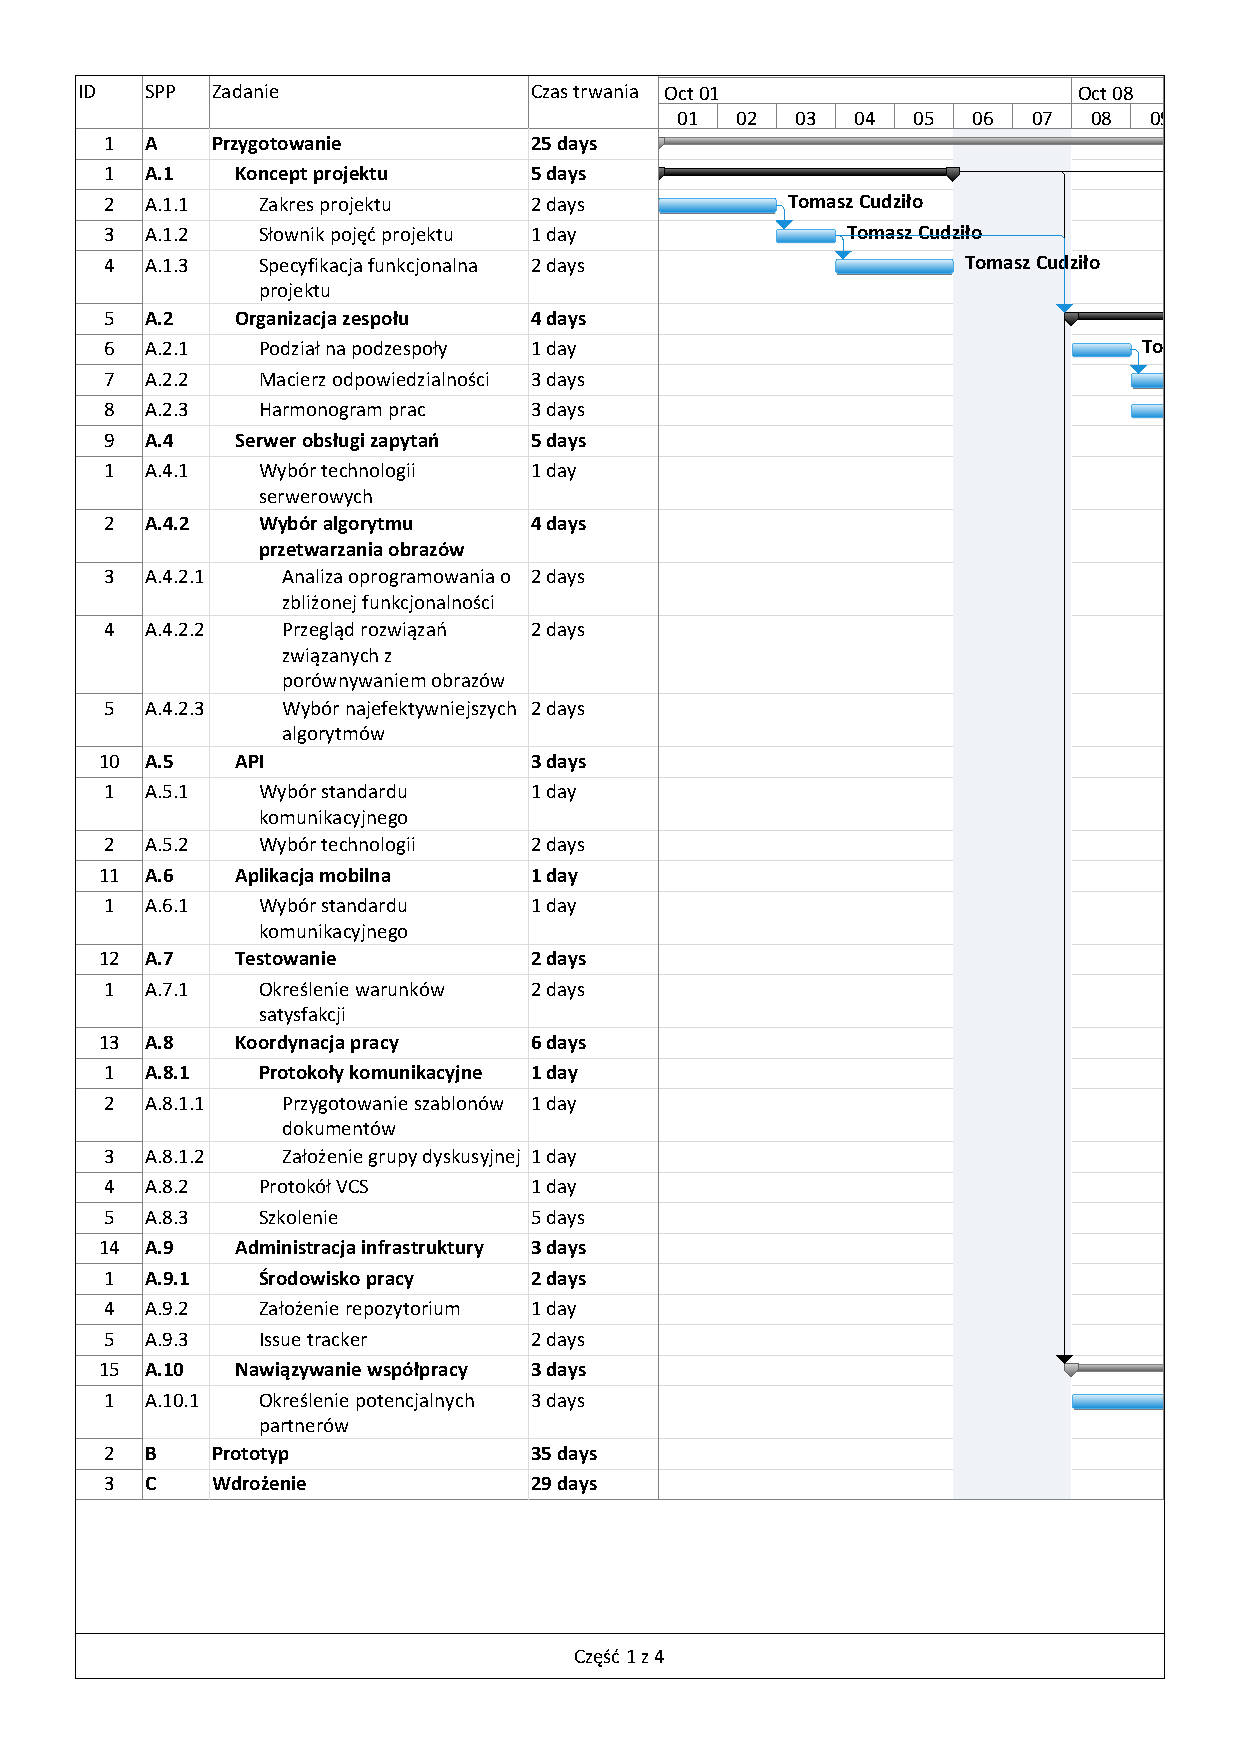
\includegraphics[trim=1.2cm 1.2cm 1.2cm 1.2cm,page=1,width=\textwidth]{./figury/harmonogram/harmonogram-pracy-A-przygotowanie}
    \caption{Harmonogram pracy iteracji \emph{Przygotowanie} projektu \emph{Concerto}.}
    \label{fig:harmonogram:iteracja_przygotowanie}
\end{figure}

\begin{figure}[p]
    \ContinuedFloat
    \includegraphics[trim=1.2cm 1.2cm 1.2cm 1.2cm,page=2,width=\textwidth]{./figury/harmonogram/harmonogram-pracy-A-przygotowanie}
    \caption[]{Harmonogram pracy iteracji \emph{Przygotowanie} projektu \emph{Concerto}. (kontynuacja)}
\end{figure}

\begin{figure}[p]
    \ContinuedFloat
    \includegraphics[trim=1.2cm 1.2cm 1.2cm 1.2cm,page=3,width=\textwidth]{./figury/harmonogram/harmonogram-pracy-A-przygotowanie}
    \caption[]{Harmonogram pracy iteracji \emph{Przygotowanie} projektu \emph{Concerto}. (kontynuacja)}
\end{figure}

\begin{figure}[p]
    \ContinuedFloat
    \includegraphics[trim=1.2cm 1.2cm 1.2cm 1.2cm,page=4,width=\textwidth]{./figury/harmonogram/harmonogram-pracy-A-przygotowanie}
    \caption[]{Harmonogram pracy iteracji \emph{Przygotowanie} projektu \emph{Concerto}. (kontynuacja)}
\end{figure}

\subsubsection{Iteracja B -- Prototyp}
Zadania iteracji B mają na celu stworzenie produktów oferujących jedynie
funkcjonalność krytyczną dla projektu. Iteracja B zaczyna się 5. listopada 2012
i kończy 21. grudnia 2012 r. Zakładany budżet to 53 000 PLN. Harmonogram prac
nad zadaniami iteracji \emph{Prototyp} zaczyna się na stronie
\pageref{fig:harmonogram:iteracja_prototyp}.

\begin{figure}[p]
    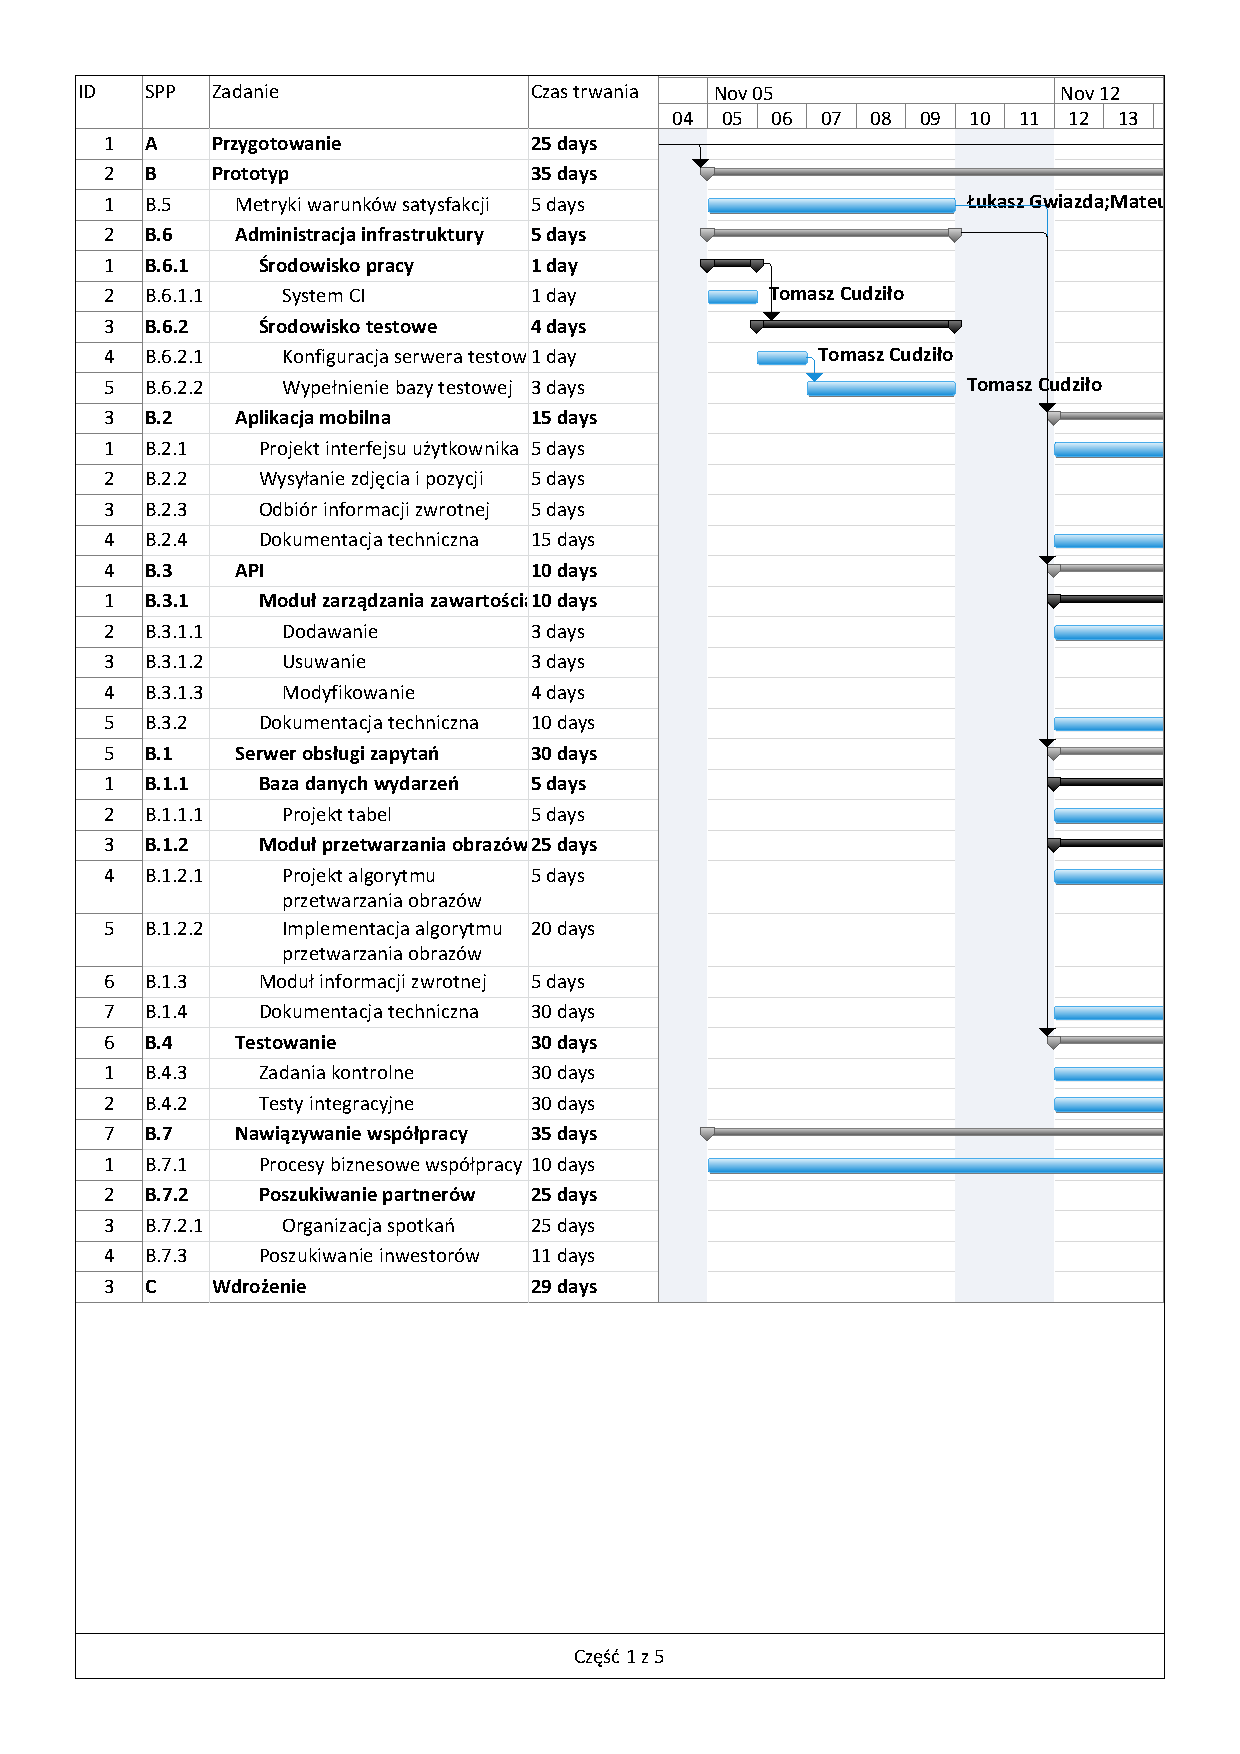
\includegraphics[trim=1.2cm 1.2cm 1.2cm 1.2cm, page=1, width=\textwidth]{./figury/harmonogram/harmonogram-pracy-B-prototyp}
    \caption{Harmonogram pracy iteracji \emph{Protyp} projektu \emph{Concerto}.}
    \label{fig:harmonogram:iteracja_prototyp}
\end{figure}

\begin{figure}[p]
    \ContinuedFloat
    \includegraphics[trim=1.2cm 1.2cm 1.2cm 1.2cm, page=2, width=\textwidth]{./figury/harmonogram/harmonogram-pracy-B-prototyp}
    \caption[]{Harmonogram pracy iteracji \emph{Prototyp} projektu \emph{Concerto}. (kontynuacja)}
\end{figure}

\begin{figure}[p]
    \ContinuedFloat
    \includegraphics[trim=1.2cm 1.2cm 1.2cm 1.2cm, page=3, width=\textwidth]{./figury/harmonogram/harmonogram-pracy-B-prototyp}
    \caption[]{Harmonogram pracy iteracji \emph{Prototyp} projektu \emph{Concerto}. (kontynuacja)}
\end{figure}

\begin{figure}[p]
    \ContinuedFloat
    \includegraphics[trim=1.2cm 1.2cm 1.2cm 1.2cm, page=4, width=\textwidth]{./figury/harmonogram/harmonogram-pracy-B-prototyp}
    \caption[]{Harmonogram pracy iteracji \emph{Prototyp} projektu \emph{Concerto}. (kontynuacja)}
\end{figure}

\begin{figure}[p]
    \ContinuedFloat
    \includegraphics[trim=1.2cm 1.2cm 1.2cm 1.2cm, page=5, width=\textwidth]{./figury/harmonogram/harmonogram-pracy-B-prototyp}
    \caption[]{Harmonogram pracy iteracji \emph{Prototyp} projektu \emph{Concerto}. (kontynuacja)}
\end{figure}

\subsubsection{Iteracja C -- Wdrożenie}
Prace iteracji C zaczynają się 3. stycznia 2013, a kończą 12. lutego 2013.
Budżet iteracji to 57 000 PLN. Harmonogram przydziału zadań iteracji
\emph{Wdrożenie} zaczyna się na stronie
\pageref{fig:harmonogram:iteracja_wdrozenie}.

\begin{figure}[p]
    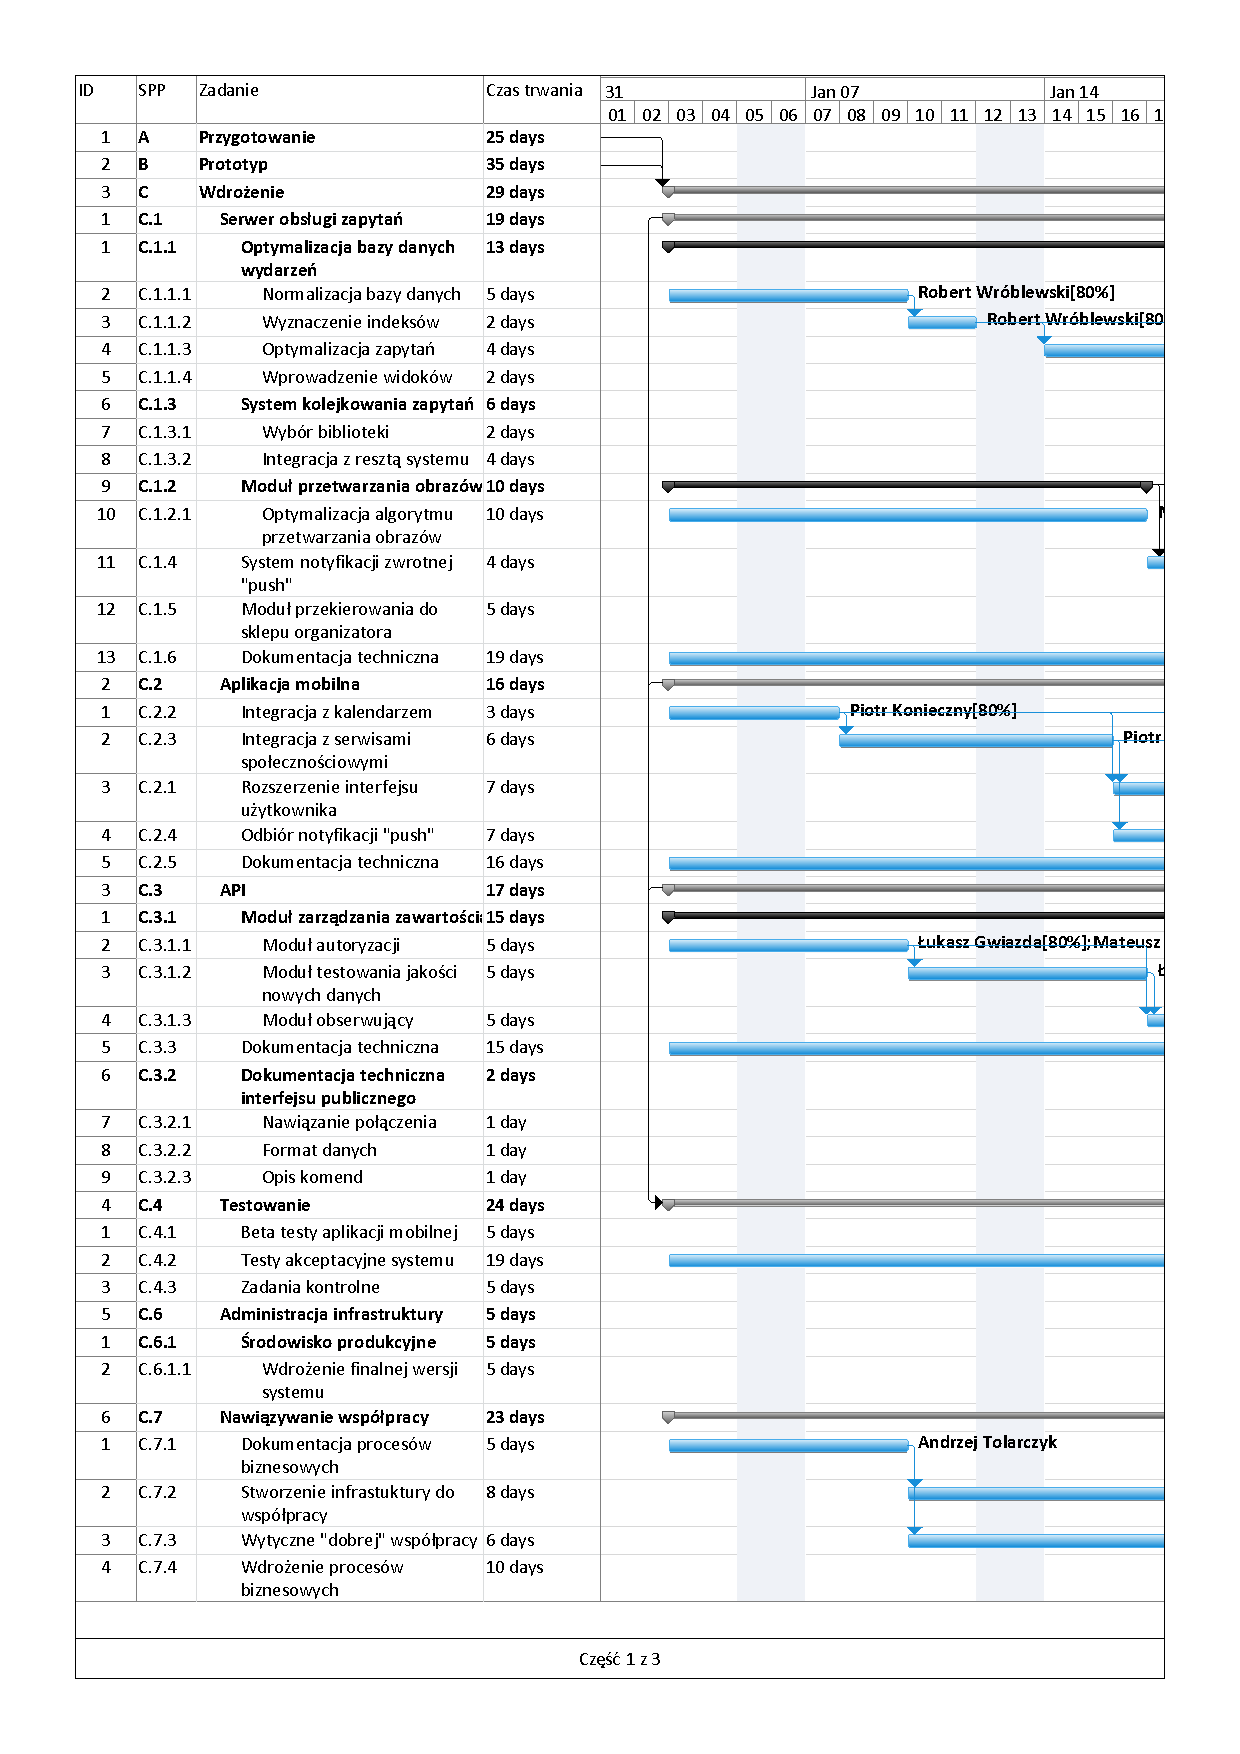
\includegraphics[trim=1.2cm 1.2cm 1.2cm 1.2cm, page=1, width=\textwidth]{./figury/harmonogram/harmonogram-pracy-C-wdrozenie}
    \caption{Harmonogram pracy iteracji \emph{Wdrożenie} projektu \emph{Concerto}.}
    \label{fig:harmonogram:iteracja_wdrozenie}
\end{figure}

\begin{figure}[p]
    \ContinuedFloat
    \includegraphics[trim=1.2cm 1.2cm 1.2cm 1.2cm, page=2, width=\textwidth]{./figury/harmonogram/harmonogram-pracy-C-wdrozenie}
    \caption[]{Harmonogram pracy iteracji \emph{Wdrożenie} projektu \emph{Concerto}. (kontynuacja)}
\end{figure}

\begin{figure}[p]
    \ContinuedFloat
    \includegraphics[trim=1.2cm 1.2cm 1.2cm 1.2cm, page=3, width=\textwidth]{./figury/harmonogram/harmonogram-pracy-C-wdrozenie}
    \caption[]{Harmonogram pracy iteracji \emph{Wdrożenie} projektu \emph{Concerto}. (kontynuacja)}
\end{figure}
